\documentclass{article}


\usepackage[utf8]{inputenc} % allow utf-8 input
\usepackage[T1]{fontenc}    % use 8-bit T1 fonts
\usepackage{hyperref}       % hyperlinks
\usepackage{url}            % simple URL typesetting
\usepackage{booktabs}       % professional-quality tables
\usepackage{amsfonts}       % blackboard math symbols
\usepackage{nicefrac}       % compact symbols for 1/2, etc.
\usepackage{microtype}      % microtypography
\usepackage{lipsum}
\usepackage{graphicx}

\title{Deep Reinforcement Learning Udacity ND: Navigation Project}

\author{%
  Nicolas Benielli Borrajo \\
  \texttt{https://github.com/thenickben} \\
    }

\begin{document}

\maketitle

\begin{abstract}
 In this project I study the behaviour of two Deep Reinforcement Learning algorithms: DQN and Double-DQN. The environment correspond to the Banana Collector from Unity. I particularly study the impact of small changes in both network architecture and learning hyperparameters, with the goal of solving the problem in the lowest number of training episodes such that the average reward, over a 100-steps time-sliding window, is greater than $13.1$. The best model found is a DQN with Batch Normalization that is able to solve the environment in only 239 steps. I found that the learning curves can be optimized for both learning algorithms but their optimal hyperparameters are not necessarily the same, which imposes difficulties on their direct comparison. Also, I found that introducing some form of regularization in the neural network can boost the learning process.  
\end{abstract}

%---------------------------------------------------------------------------------------------
\section{Introduction}

Deep Reinforcement Learning (DRL) studies the application of deep learning techniques (such as deep neural networks) to the problem of value function approximation in large scale reinforcement learning environments. In the early stages of reinforcement learning research, tabular-based methods were used to exactly solve either the state-value function $v(s)$ or the action-value function $q(s,a)$ for an agent interacting with an environment within a Markov Decision Process (MDP) \footnote{Solve meaning to obtain the optimal policy $\pi_{(s,a)}^*}$ that maps each state $s$ with an optimal action $a$}  . However, when the action or state spaces are large, the representation of optimal policies through simple \textit{v-lookup} table methods becomes infeasible and suffers from the well-known curse of dimensionality. Hence, researchers developed approximate methods for estimating $q(s,a)$ through function approximation methods. In this work I implement two of these approaches, known as DQN [1] and Double-DQN [2] to estimate optimal action-value functions for 3D Unity environment Banana Collector [5].

Some improvements to the vanilla DQN algorithm I considered here as follows:

\begin{itemize}
	\item Soft updates: instead updating the target network as a "hard" copy of the q-network, we use a similar approach as in DDPG [4] known as soft-updates.
	\item Batch normalization, which was introduced later than the original DQN paper, and has been incorporated in DDPG.
	\item Maximization bias, also known as the double-DQN algorithm.
\end{itemize}

It worth to notice that DQN only works for low dimensional discrete action spaces (such as those in Atari games). In the case of continuous action spaces, other approaches like Policy Gradient methods (DDPG for example) are commonly used.

\subsection{Problem Description}

The MDP to solve is the Banana Collector environment from Unity [5], a 3D room  where there are yellow and blue bananas randomly located. The agent is free to move across the room, obtaining a reward of $+1$ when collecting a yellow banana, $-1$ when collecting a blue one, and zero otherwise. The state space has 37 dimensions and contains the agent’s velocity, along with a ray-based perception of objects around agent’s forward direction. The action space consists in four discrete actions, corresponding to moving forward, backward, turn left and turn right. The environment is considered to being solved when the average reward, over a sliding window of 100 steps wide, is equal or greater than $13.1$. 

\section{Experimental Methods}

\subsection{Methodology}

The solution was implemented in Python using the PyTorch library for handling the optimization of the neural networks through backpropagation. The implementation of the methods follows the algorithm presented in [1]for the \textit{vanilla} DQN, using a \textit{soft update} for the target network as proposed in [4]. The exploration was implemented using an $\epsilon$-greedy algorithm with exponential decay and a minimum of $\epsilon = 0.01$.

\subsection{Network Architecture}

The neural network used for function approximation is a simple 2 fully-connected linear layers of dimensions $fc1_{units}$ and $fc2_{units}$ with ReLu activations, and an intermediate Batch Normalization layer that can be switched ON/OFF according to a boolean flag. 

\subsection{Base Case Hyperparameters}

In order to test whether my implemented agent is able to learn from training, I chose a set of hyperparameters following some intuition about their commonly used values. In particular, given the dimension of the state space, I expect that a network with $fc1_{units} = 32$ and $fc1_{units} = 64$ should be enough to converge to the optimal value function. The base case hyperparameter values for DQN are shown in Table 1. The same values were used as base case for Double-DQN.

\begin{table}[h!]
\centering
\begin{tabular}{ll}
\toprule
Hyperparameter &      Value \\
\midrule
           ALGORITHM &      dqn \\
 TRAIN\_EPISODES &     1000 \\
    BUFFER\_SIZE &  1000000 \\
     BATCH\_SIZE &       64 \\
          GAMMA &     0.99 \\
            TAU &    0.001 \\
       EPS\_INIT &      1.0 \\
      EPS\_DECAY &    0.995 \\
             LR &    0.001 \\
   UPDATE\_EVERY &        5 \\
      ACT\_EVERY &        1 \\
            FC1 &       32 \\
            FC2 &       64 \\
             BN &     True \\
           SEED &       42 \\
\bottomrule
\end{tabular}
\label{table:base_case}
\caption{Hyperparameters for the base case.}
\end{table}


\subsection{Hyperparameters Tuning}

The set of hyperparameters and values shown in Table 2 were used to train a different model for each possible combination, resulting in a total of 160 training instances. The rest of the learning and network hyperparameters are held fixed across all models (as shown in Table 1). 

\begin{table}[h!]
\centering
\begin{tabular}{ll}
\toprule
\midrule
Algorithm  &  ['ddqn', 'ddqn'] \\
Batch size &  [32, 64, 128, 256] \\
Learning rate &  [0.01, 0.005, 0.001, 0.0005, 0.0001] \\
Initial $\epsilon$ &  [1.0, 0.5] \\
$\epsilon$ Decay rate &  [0.99, 0.995] \\
\bottomrule
\end{tabular}
\label{table:hyperp}
\caption{Hyperparameters values for tuning.}
\end{table}

%---------------------------------------------------------------------------------------------
\section{Results}

\subsection{Analysis}

The base case results are shown in Figure 1 and Table 3. At a first glance it can be seen that the problem is considered solved for all cases. It worth to mention that the plots finishes when the average reward is greater than 13.1; thus in the cases where training "stops" earlier than others it means that they reach the goal faster. In fact, the scoring value I use to compare different algorithms and settings is the number of steps needed to reach this goal (the lower, the better). Table 3 shows the necessary steps to solve the environment for each case, alongside with the final $\epsilon$ in order to take into account the importance of its decay during the learning process.

Even if it seems that not including a Batch Normalization layer can potentially help to improve the learning rate (as in the case of Double-DQN in the base case), by doing a further change in hyperparameters I concluded that, on average, Batch Normalization helps to achieve faster learning. Thus, I will only consider the case where Batch Normalization is applied for further hyperparameters tuning (this means, in Table 2 all cases correspond to applying batch normalization).

In Figure 2 there are shown the learning curves for the base case and best models, where it becomes evident that a careful hyperparameter tuning can drastically improve learning.

Table 6 in Appendix show all the results for the different test cases, and their corresponding hyperparameters and learning curves are provided in the project github. I found that the best model is a DQN, that is able to solve the environment in 234 steps and where its set of hyperparameters are the ones shown in Table 4. On the other hand, the best DDQN model was able to solve the environment in 274 steps, and its hyperparameters are shown in Table 5. The test cases where the steps are shown as 1000 correspond to configurations not able to solve the environment in less than such an amount of episodes. 

\begin{figure}[h!]
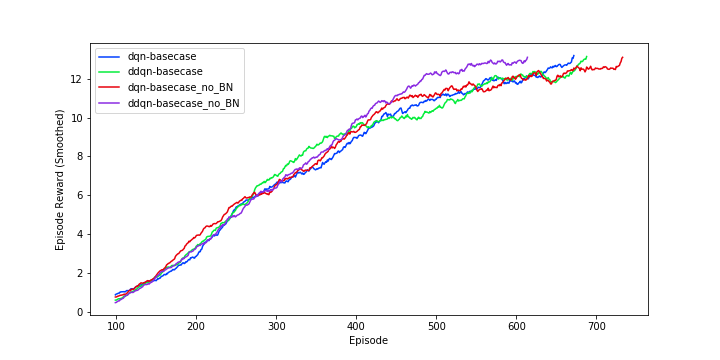
\includegraphics[width=15cm]{basecase-plot.png}
\centering
\caption{Base case models results}
\label{fig:mesh1}
\end{figure}

\begin{figure}[h!]
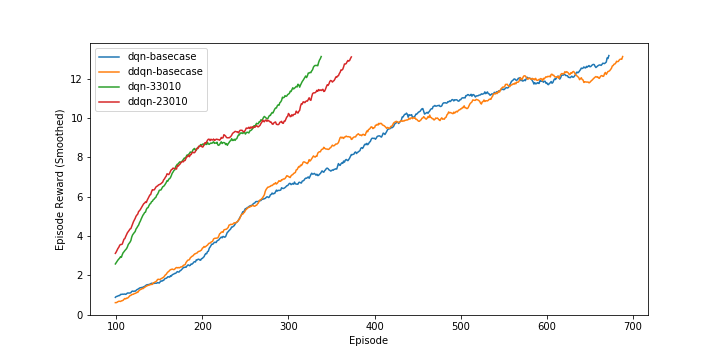
\includegraphics[width=15cm]{best_vs_basecase-plot.png}
\centering
\caption{Best vs base case models results}
\label{fig:mesh1}
\end{figure}

\begin{table}[h!]
\centering
\begin{tabular}{lcc}
\toprule
Test name & Steps to solve  & Final  $\epsilon$ \\
\midrule
ddn-basecase &  673 &	0.034272 \\
dqn-basecase(no BN)  & 734 & 0.025243\\
ddqn-basecase & 689  & 0.031630 \\
ddqn-basecase (no BN)  & 615 &  0.045835 \\
ddq-best & 234  & 0.016569 \\
ddqn-best & 274 &  0.011655 \\
\bottomrule
\end{tabular}
\label{table:res_basecase}
\caption{Results for the base cases.}
\end{table}

\begin{table}[h!]
\centering
\begin{tabular}{ll}
\toprule
           Hyperparameter &      Value \\
\midrule
           ALGO &      dqn \\
 TRAIN\_EPISODES &     1000 \\
    BUFFER\_SIZE &  1000000 \\
     BATCH\_SIZE &      256 \\
          GAMMA &     0.99 \\
            TAU &    0.001 \\
       EPS\_INIT &      0.5 \\
      EPS\_DECAY &     0.99 \\
             LR &   0.0005 \\
   UPDATE\_EVERY &        5 \\
      ACT\_EVERY &        1 \\
            FC1 &       32 \\
            FC2 &       64 \\
             BN &     True \\
           SEED &       42 \\
\bottomrule
\end{tabular}
\label{table:res_basecase}
\caption{Hyperparameters for the best model, solving the environment in 239 steps}
\end{table}

\begin{table}[h!]
\centering
\begin{tabular}{ll}
\toprule
           Hyperparameter &      Value \\
\midrule
ALGO &     DDQN \\
 TRAIN\_EPISODES &     1000 \\
    BUFFER\_SIZE &  1000000 \\
     BATCH\_SIZE &      128 \\
          GAMMA &     0.99 \\
            TAU &    0.001 \\
       EPS\_INIT &      0.5 \\
      EPS\_DECAY &     0.99 \\
             LR &   0.0005 \\
   UPDATE\_EVERY &        5 \\
      ACT\_EVERY &        1 \\
            FC1 &       32 \\
            FC2 &       64 \\
             BN &     True \\
           SEED &       42 \\
\bottomrule
\end{tabular}
\label{table:res_basecase}
\caption{Hyperparameters for the best DDQN model, solving the environment in 274 steps}
\end{table}

\subsection{Discussion and Further work}

In this work I implemented a DQN algorithm to solve the Unity environment known as Banana Collector. I explored different hyperparameters and modifications to the vanilla DQN algorithm. I found that the best model turned to be a DQN with Batch Normalization and soft updates after a careful hyperparameter tuning. As a future improvements to this model, it worth to explore other family of modifications such as Prioritized Experience Replay, Noisy networks and n-step returns, which are all taken into account in one of the state of the art DRL models known as Rainbow [3].


\section*{References}

\small

[1] Mnih, V. et al \ (2015) Human-level control through
deep reinforcement learning. \textit{ Nature }, 518(7540):529–533. \\

\noindent
[2] van Hasselt, H.\ \& Guez, A.\ \& and Silver, D. \ (2016) Deep reinforcement learning with double Q-learning.\ \textit{ Proc. of AAAI}, 2094–2100.\\

\noindent
[3] Hessel, M. et al. \ (2017) Rainbow: Combining Improvements in Deep Reinforcement Learning. \ \textit{Thirty-Second AAAI Conference on Artificial Intelligence}\\

\noindent
[4] Lillicrap, T. et al \ (2016) Continuous control with deep reinforcement learning. \ \textit{arXiv preprint}, arXiv:1509.02971 \\

\noindent
[5] Unity Technologies, ml-agents \ \textit{https://github.com/Unity-Technologies/ml-agents/} \\


\section*{Appendix: All test results during hyperparameter search}

\begin{table}
\centering
\begin{tabular}{llrrr}
\toprule
Test number &            Test\_name &  Steps\_to\_solve &  Final\_eps &  Episodes\_min\_eps \\
\midrule
0   &            dqn-00000 &            1000 &   0.010000 &               459 \\
1   &            dqn-00001 &            1000 &   0.010000 &               919 \\
2   &            dqn-00010 &            1000 &   0.010000 &               390 \\
3   &            dqn-00011 &            1000 &   0.010000 &               781 \\
4   &            dqn-01000 &            1000 &   0.010000 &               459 \\
5   &            dqn-01001 &            1000 &   0.010000 &               919 \\
6   &            dqn-01010 &             466 &   0.010000 &               390 \\
7   &            dqn-01011 &            1000 &   0.010000 &               781 \\
8   &            dqn-02000 &             387 &   0.010000 &               459 \\
9   &            dqn-02001 &             498 &   0.049912 &              1000 \\
10  &            dqn-02010 &             302 &   0.010000 &               390 \\
11  &            dqn-02011 &             380 &   0.045087 &              1000 \\
12  &            dqn-03000 &             434 &   0.010000 &               459 \\
13  &            dqn-03001 &             475 &   0.056011 &              1000 \\
14  &            dqn-03010 &             330 &   0.010000 &               390 \\
15  &            dqn-03011 &             426 &   0.035802 &              1000 \\
16  &            dqn-04000 &             451 &   0.010000 &               459 \\
17  &            dqn-04001 &             725 &   0.015997 &              1000 \\
18  &            dqn-04010 &             460 &   0.010000 &               390 \\
19  &            dqn-04011 &             490 &   0.025977 &              1000 \\
20  &            dqn-10000 &            1000 &   0.010000 &               459 \\
21  &            dqn-10001 &            1000 &   0.010000 &               919 \\
22  &            dqn-10010 &            1000 &   0.010000 &               390 \\
23  &            dqn-10011 &            1000 &   0.010000 &               781 \\
24  &            dqn-11000 &             477 &   0.010000 &               459 \\
25  &            dqn-11001 &            1000 &   0.010000 &               919 \\
26  &            dqn-11010 &            1000 &   0.010000 &               390 \\
27  &            dqn-11011 &             509 &   0.023617 &              1000 \\
28  &            dqn-12000 &             370 &   0.010000 &               459 \\
29  &            dqn-12001 &             466 &   0.058595 &              1000 \\
30  &            dqn-12010 &             365 &   0.010000 &               390 \\
31  &            dqn-12011 &             379 &   0.045313 &              1000 \\
32  &            dqn-13000 &             405 &   0.010000 &               459 \\
33  &            dqn-13001 &             438 &   0.067424 &              1000 \\
34  &            dqn-13010 &             343 &   0.010000 &               390 \\
35  &            dqn-13011 &             397 &   0.041404 &              1000 \\
36  &            dqn-14000 &             452 &   0.010000 &               459 \\
37  &            dqn-14001 &             573 &   0.034272 &              1000 \\
38  &            dqn-14010 &             391 &   0.010000 &               390 \\
39  &            dqn-14011 &             489 &   0.026107 &              1000 \\
40  &            dqn-20000 &            1000 &   0.010000 &               459 \\
41  &            dqn-20001 &            1000 &   0.010000 &               919 \\
42  &            dqn-20010 &            1000 &   0.010000 &               390 \\
43  &            dqn-20011 &            1000 &   0.010000 &               781 \\
44  &            dqn-21000 &             375 &   0.010000 &               459 \\
45  &            dqn-21001 &             820 &   0.010000 &               919 \\
46  &            dqn-21010 &             416 &   0.010000 &               390 \\
47  &            dqn-21011 &             692 &   0.010000 &               781 \\
48  &            dqn-22000 &             319 &   0.014830 &              1000 \\
49  &            dqn-22001 &             471 &   0.057145 &              1000 \\
50  &            dqn-22010 &             284 &   0.010541 &              1000 \\
\bottomrule
\end{tabular}
\label{table:res_basecase}
\caption{Model results for hyperparameters tuning (a)}
\end{table}

\begin{table}
\centering
\begin{tabular}{llrrr}
\toprule
Test number &            Test\_name &  Steps\_to\_solve &  Final\_eps &  Episodes\_min\_eps \\
\midrule
51  &            dqn-22011 &             351 &   0.052141 &              1000 \\
52  &            dqn-23000 &             356 &   0.010225 &              1000 \\
53  &            dqn-23001 &             448 &   0.064128 &              1000 \\
54  &            dqn-23010 &             303 &   0.010000 &               390 \\
55  &            dqn-23011 &             370 &   0.047404 &              1000 \\
56  &            dqn-24000 &             344 &   0.011535 &              1000 \\
57  &            dqn-24001 &             577 &   0.033591 &              1000 \\
58  &            dqn-24010 &             304 &   0.010000 &               390 \\
59  &            dqn-24011 &             442 &   0.033043 &              1000 \\
60  &            dqn-30000 &             449 &   0.010000 &               459 \\
61  &            dqn-30001 &             698 &   0.018315 &              1000 \\
62  &            dqn-30010 &             419 &   0.010000 &               390 \\
63  &            dqn-30011 &            1000 &   0.010000 &               781 \\
64  &            dqn-31000 &            1000 &   0.010000 &               459 \\
65  &            dqn-31001 &             678 &   0.020247 &              1000 \\
66  &            dqn-31010 &             643 &   0.010000 &               390 \\
67  &            dqn-31011 &             602 &   0.014817 &              1000 \\
68  &            dqn-32000 &             349 &   0.010970 &              1000 \\
69  &            dqn-32001 &             470 &   0.057432 &              1000 \\
70  &            dqn-32010 &             315 &   0.010000 &               390 \\
71  &            dqn-32011 &             391 &   0.042668 &              1000 \\
72  &            dqn-33000 &             457 &   0.010000 &               459 \\
73  &            dqn-33001 &             470 &   0.057432 &              1000 \\
74  &            dqn-33010 &             239 &   0.016569 &              1000 \\
75  &            dqn-33011 &             387 &   0.043532 &              1000 \\
76  &            dqn-34000 &             343 &   0.011652 &              1000 \\
77  &            dqn-34001 &             443 &   0.065756 &              1000 \\
78  &            dqn-34010 &             288 &   0.010126 &              1000 \\
79  &            dqn-34011 &             356 &   0.050850 &              1000 \\
80  &           ddqn-00000 &            1000 &   0.010000 &               459 \\
81  &           ddqn-00001 &            1000 &   0.010000 &               919 \\
82  &           ddqn-00010 &            1000 &   0.010000 &               390 \\
83  &           ddqn-00011 &            1000 &   0.010000 &               781 \\
84  &           ddqn-01000 &            1000 &   0.010000 &               459 \\
85  &           ddqn-01001 &             650 &   0.023298 &              1000 \\
86  &           ddqn-01010 &            1000 &   0.010000 &               390 \\
87  &           ddqn-01011 &            1000 &   0.010000 &               781 \\
88  &           ddqn-02000 &             355 &   0.010328 &              1000 \\
89  &           ddqn-02001 &             513 &   0.046297 &              1000 \\
90  &           ddqn-02010 &             304 &   0.010000 &               390 \\
91  &           ddqn-02011 &             350 &   0.052403 &              1000 \\
92  &           ddqn-03000 &             401 &   0.010000 &               459 \\
93  &           ddqn-03001 &             475 &   0.056011 &              1000 \\
94  &           ddqn-03010 &             312 &   0.010000 &               390 \\
95  &           ddqn-03011 &             358 &   0.050343 &              1000 \\
96  &           ddqn-04000 &             403 &   0.010000 &               459 \\
97  &           ddqn-04001 &             537 &   0.041049 &              1000 \\
98  &           ddqn-04010 &             413 &   0.010000 &               390 \\
99  &           ddqn-04011 &             568 &   0.017571 &              1000 \\
100 &           ddqn-10000 &            1000 &   0.010000 &               459 \\
\bottomrule
\end{tabular}
\label{table:res_basecase}
\caption{Model results for hyperparameters tuning (b)}
\end{table}

\begin{table}
\centering
\begin{tabular}{llrrr}
\toprule
Test number &            Test\_name &  Steps\_to\_solve &  Final\_eps &  Episodes\_min\_eps \\
\midrule
101 &           ddqn-10001 &            1000 &   0.010000 &               919 \\
102 &           ddqn-10010 &            1000 &   0.010000 &               390 \\
103 &           ddqn-10011 &            1000 &   0.010000 &               781 \\
104 &           ddqn-11000 &             776 &   0.010000 &               459 \\
105 &           ddqn-11001 &             889 &   0.010000 &               919 \\
106 &           ddqn-11010 &             389 &   0.010000 &               390 \\
107 &           ddqn-11011 &            1000 &   0.010000 &               781 \\
108 &           ddqn-12000 &             356 &   0.010225 &              1000 \\
109 &           ddqn-12001 &             550 &   0.038459 &              1000 \\
110 &           ddqn-12010 &             318 &   0.010000 &               390 \\
111 &           ddqn-12011 &             335 &   0.056495 &              1000 \\
112 &           ddqn-13000 &             341 &   0.011888 &              1000 \\
113 &           ddqn-13001 &             546 &   0.039238 &              1000 \\
114 &           ddqn-13010 &             390 &   0.010000 &               390 \\
115 &           ddqn-13011 &             445 &   0.032550 &              1000 \\
116 &           ddqn-14000 &             385 &   0.010000 &               459 \\
117 &           ddqn-14001 &             589 &   0.031630 &              1000 \\
118 &           ddqn-14010 &             450 &   0.010000 &               390 \\
119 &           ddqn-14011 &             547 &   0.019521 &              1000 \\
120 &           ddqn-20000 &            1000 &   0.010000 &               459 \\
121 &           ddqn-20001 &            1000 &   0.010000 &               919 \\
122 &           ddqn-20010 &            1000 &   0.010000 &               390 \\
123 &           ddqn-20011 &            1000 &   0.010000 &               781 \\
124 &           ddqn-21000 &             858 &   0.010000 &               459 \\
125 &           ddqn-21001 &             874 &   0.010000 &               919 \\
126 &           ddqn-21010 &            1000 &   0.010000 &               390 \\
127 &           ddqn-21011 &             454 &   0.031114 &              1000 \\
128 &           ddqn-22000 &             400 &   0.010000 &               459 \\
129 &           ddqn-22001 &             496 &   0.050415 &              1000 \\
130 &           ddqn-22010 &             400 &   0.010000 &               390 \\
131 &           ddqn-22011 &             441 &   0.033209 &              1000 \\
132 &           ddqn-23000 &             333 &   0.012884 &              1000 \\
133 &           ddqn-23001 &             542 &   0.040033 &              1000 \\
134 &           ddqn-23010 &             274 &   0.011656 &              1000 \\
135 &           ddqn-23011 &             402 &   0.040379 &              1000 \\
136 &           ddqn-24000 &             360 &   0.010000 &               459 \\
137 &           ddqn-24001 &             556 &   0.037320 &              1000 \\
138 &           ddqn-24010 &             276 &   0.011424 &              1000 \\
139 &           ddqn-24011 &             404 &   0.039976 &              1000 \\
140 &           ddqn-30000 &            1000 &   0.010000 &               459 \\
141 &           ddqn-30001 &            1000 &   0.010000 &               919 \\
142 &           ddqn-30010 &            1000 &   0.010000 &               390 \\
143 &           ddqn-30011 &            1000 &   0.010000 &               781 \\
144 &           ddqn-31000 &             711 &   0.010000 &               459 \\
145 &           ddqn-31001 &             762 &   0.013289 &              1000 \\
146 &           ddqn-31010 &             308 &   0.010000 &               390 \\
147 &           ddqn-31011 &             371 &   0.047167 &              1000 \\
148 &           ddqn-32000 &             440 &   0.010000 &               459 \\
149 &           ddqn-32001 &             559 &   0.036763 &              1000 \\
150 &           ddqn-32010 &             326 &   0.010000 &               390 \\
\bottomrule
\end{tabular}
\label{table:res_basecase}
\caption{Model results for hyperparameters tuning (c)}
\end{table}


\begin{table}
\begin{tabular}{llrrr}
\toprule
Test number &            Test\_name &  Steps\_to\_solve &  Final\_eps &  Episodes\_min\_eps \\
\midrule
151 &           ddqn-32011 &             513 &   0.023148 &              1000 \\
152 &           ddqn-33000 &             473 &   0.010000 &               459 \\
153 &           ddqn-33001 &             417 &   0.074909 &              1000 \\
154 &           ddqn-33010 &             347 &   0.010000 &               390 \\
155 &           ddqn-33011 &             445 &   0.032550 &              1000 \\
156 &           ddqn-34000 &             386 &   0.010000 &               459 \\
157 &           ddqn-34001 &             464 &   0.059186 &              1000 \\
158 &           ddqn-34010 &             347 &   0.010000 &               390 \\
159 &           ddqn-34011 &             387 &   0.043532 &              1000 \\
160 &         dqn-basecase &             573 &   0.034272 &              1000 \\
161 &   dqn-basecase\_no\_BN &             634 &   0.025243 &              1000 \\
162 &        ddqn-basecase &             589 &   0.031630 &              1000 \\
163 &  ddqn-basecase\_no\_BN &             515 &   0.045835 &              1000 \\
164 &        ddqn-bestnoBN &             280 &   0.010973 &              1000 \\
\bottomrule
\end{tabular}
\label{table:res_basecase}
\caption{Model results for hyperparameters tuning (d)}
\end{table}



\end{document}
